\documentclass[12pt,a4paper]{article}
\usepackage[utf8]{inputenc}
\usepackage{amsmath}
\usepackage{amsfonts}
\usepackage{amssymb}
\usepackage{epsfig}
\usepackage[linesnumbered,ruled,vlined]{algorithm2e}
\usepackage[left=2cm,right=2cm,top=2cm,bottom=2cm]{geometry}

\usepackage{pgf, tikz}
\usepackage{color}
\usepackage{listings}
\usepackage{verbatim}
\usepackage{array}
\usepackage{float}
\usepackage{capt-of}
\usepackage{inputenc}

\author{Romain Pascual et Adam Hotait}
\date{22 Janvier 2019}
\title{Devoir Maison d'Optimisation: Clustering}
\begin{document}

\maketitle

\section*{Présentation du problème}
On considère l'île de Man. Le fichier proposé décrit son réseau routier sous forme de graphe orienté, dont les sommets sont les intersections et les arcs des routes entre deux intersections, pondérés par le temps de trajet. Afin de simplifier le projet, nous supposons que les routes sont navigables dans les deux sens et on se restreint aux sommets dont les coordonnées GPS sont entre $54.0790$ et $54.1549$ pour la longitude et entre $-5$ et $-4.7364$ pour la latitude. On obtient ainsi un graph composé de $345$ sommets. Il décrit une  métrique sur l'espace des sommets $V$ telle que la distance $d_{u,v}$ entre les sommets $u$ et $v$ décrit la longueur du plus court chemin entre ces deux sommets. Le filtrage utilisé sépare le graphe en différentes composantes connexes. Ainsi on définit arbitrairement $1e9$ comme la distance entre deux sommets non connectés. Cette valeur est très grande devant toutes les distances considérées et peut donc être considérée come $\infty$. Les distances ont été précalculées et sont donc fournies.

Il s'agit de résoudre trois problèmes : le problème $k$-médiane, le problème $k$-moyenne et le problème $k$-centre. Il s'agit de trois problèmes de clustering pour lesquels on cherche $k$ sommets $\{c_1, \dots c_{k}\}$ qui minimize une fonction cible liée aux distances entres les points et le centre de leur cluster.

\paragraph{$k$-médiane} On cherche la liste des $k$ sommets qui minimise :

\[ k\_median(G) = \sum_{v \in V} \min_i d_{c_i,v} \].

\paragraph{$k$-moyenne} On cherche la liste des $k$ sommets qui minimise :

\[ k\_mean(G) = \sum_{v \in V} \min_i d^{2}_{c_i,v} \].

\paragraph{$k$-centre} On cherche la liste des $k$ sommets qui minimise :

\[ k\_center(G) = \max_{v \in V} \min_i d_{c_i,v} \].

\section*{Résolution}
Etant donné que les trois problèmes sont essentiellement identiques, la formulation sout la forme d'un programme lineaire est la même, seule la fonction à minimiser diffère.

Tout d'abord, reformulons le problème linéaire. Sans perte de généralité, on s'intéresse à la fonction de coût du problème $k$-médiane. On dispose en entrée d'un graphe $G = (V,E)$ non orienté, $d: E \rightarrow \mathbb{R}^+$ et on cherche :

\[ min \sum_{e = uv \in E} d(e) * x(e) * y(v) \]

tel que

\begin{alignat}{3}
& \sum_{v} y(v) \leq k & \\
& x(e) \leq y(v) & \forall e = uv \in E  \\
& \sum_{c \in V} x(uc) = 1 & \forall v \in V
\end{alignat}


Dans une telle modélisation, $x$ et $y$ sont des variables de décisions. Ainsi $y(v) = 1$ si $v$ est un centre d'un cluster et $x(uv) =1$ si $u$ appartient au cluster défini par $v$, autrement dit $v$ est le centre le plus proche de $k$.

Alors la première contrainte siginie qu'il y a au plus $k$ clusters, la deuxième signifie que $u$ ne peut être dans le cluster de $v$ que si $v$ est un centre, et la dernière assure que chaque sommet est effectivement dans un cluster. Comme on cherche à minimiser les fonctions objectifs dans chacun des cas, chaque point est bien ajouté au cluster correspondant au centre le plus proche.

Les codes des différents problèmes sont présents dans le dosser "ampl", respectivements dans les fichiers :
\begin{itemize}
\item \texttt{kmedian.mod}, 
\item \texttt{kmean.mod},
\item \texttt{kcenter.mod}.
\end{itemize}

\pagebreak
\section*{Resultats}
Voici un tableau récapitulatif des résultats obtenus pour les trois problèmes:

\begin{center}
  \begin{tabular}{ l r r l }
    \hline
    Problème & Nombre d'itération & Objectif & Centres  \\ 
    & du simplexe & & \\ \hline \hline
    $k$-median & 22771 & 1.147e7 & 283492107, 283514108, \\
    	& & & 283517728, 283523670, \\
    	& & & 456478782, 746331291 \\ \hline
    $k$-mean & 21417 & 5.268e11 & 283492107, 283502786, \\
    	& & & 283504611, 283514108, \\
    	& & & 283517728, 283523670 \\ \hline
    $k$-center & 220020 & 91044 & 283480267, 283484091, \\
    	& & &  283484618, 283508716, \\
    	& & & 283513388, 283520425\\
    \hline
  \end{tabular}
\end{center}
 
\paragraph{Analyse des résultats}

Il est à noté que pour le problème $k$-centre, la non-linéarité du $max$ nécessite une approche légèrement différente. Au lieu de chercher à minimiser 
\[ \max_{v \in V} \min_i d_{c_i,v}, \] 

\noindent on crée une variable $d$ pour laquelle on impose la contrainte

\[ \forall v \in V \min_i d_{c_i,v} \leq d. \] 

On minimise alors $d$. Cela agrandi l'espace de recherche, on obtient donc un nombre d'itération du simplexe $\simeq 10$ fois supérieur. Par ailleurs, le nombre d'itération du simplexe est accompagné de "$1$ simplex iteration for intbasis", ce qui veut dire qu'une itération suplémentaire a été nécessaire pour obtenir une solution point extrême et donc une solution entière.

\bigskip

On remarquera que les solutions aux problèmes $k$-médiane et $k$-moyennne possèdent $3$ centres en commun : $283492107$, $283517728$ et $283523670$ mais ne partagent aucun centres communs avec le problème $k$-centre. En effet, les deux premiers problèmes s'intéressent à un minimisation globale à l'intérieur d'un cluster puisque que l'on somme les contributions de tous les points, tandis que le troisième problème ne s'intéresse qu'à la contribution des points extrémaux.  

\bigskip

Par ailleurs, il est possible de visualiser les clusters en utilisant un script python. Pour ce faire, il convient tout d'abord d'exporter les solutions au format csv en utilisant ampl. Les données traitées et le script python sont présents dans le dossier "results". On obtient alors la visualisation présentée en figure \ref{fig:res}.

\begin{figure}[!ht]
\begin{center}
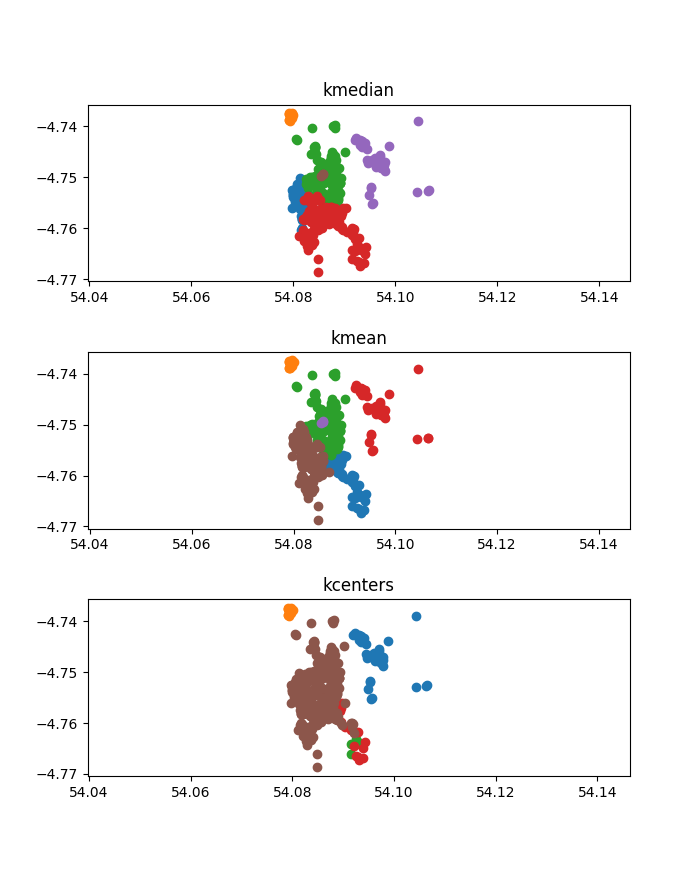
\includegraphics[width = 400 pt]{clusters.png}
\caption{Visualisation des différents clusters}
\label{fig:res}
\end{center}
\end{figure}

On remarque que les clustering pour les deux premiers premiers problèmes sont relativements similaires. Par ailleurs il est aisément possible d'isoler certaines composantes connexes (la zone en orange sur chacun des problèmes).

Cependant puisque la distance entre $2$ points n'est pas la distance euclidienne mais la distance portée par le réseau routier, ce qui revient à déformer l'espace, cette visualisation n'est pas nécessairement pertinente.

Par ailleurs, et notamment pour le problème $k$-center, de nombreux points peuvent appartenir à plusieurs clusters étant donné que leur distance à plusieurs centres est inférieure à la distance maximale. En augmentant $k$ en revanche, on améliorerait la précision, au prix d'un temps d'exécution plus long.

\end{document}